\documentclass[a4paper,12pt]{article}

\usepackage[utf8]{inputenc}
\usepackage[T1]{fontenc}
\usepackage[MeX]{polski}
\usepackage[polish]{babel}
\usepackage[latin2]{inputenc}
\usepackage[T1]{fontenc}
\usepackage{graphicx}
\usepackage{subfig}

\begin{document}
{\raggedleft{}Krzysztof Kucharczyk}\\200401\\Wydział Elektroniki\\Kierunek AiR
\\PAMSI lab. czw. 10:00-13:15\\\\\\
\begin{center} 
	\textbf{Sprawozdanie z laboratorium nr 3\\(Listy i stosy)}
\end{center}

\section{Opis zadania}

Zadanie polegało na stworzeniu pięciu algorytmów, tj. 
\begin{enumerate} 
\item Stosu na bazie tablicy (powiększanie tablicy o jedno miejsce)
\item Stosu na bazie tablicy (podwajanie tablicy)
\item Stosu na bazie listy jednokierunkowej
\item Kolejki na bazie tablicy
\item Kolejki na bazie listy jednokierunkowej

\end{enumerate}

oraz przetestowaniu wydajności dwóch pierwszych algorytmów.

\subsection{Opis algorytmu 1}

Algorytm ten miał działać jak zwykły stos. Problem przepełnienia stosu 
rozwiązany jest poprzez tworzenie nowej, większej tablicy, do której 
przepisywana jest stara tablica, a następnie usuwana. Nowa tablica zawiera
jedno miejsce dodatkowo, w które wpisywany zostaje nowy element.

Usuwanie elementu z listy następuje poprzez stworzenie mniejszej tablicy, 
do której przepisywane są elementy starej poza ostatnim, następnie stara
tablica zostaje usunięta i nadpisana nową.

\subsection{Opis algorytmu 2}

Algorytm zbudowany jest bardzo podobnie do poprzedniego, jednak tym razem 
tablica zostaje powiększona dwukrotnie w przypadku przepełnienia, natomiast
zmniejszana o połowę w przypadku gdy ilość danych wynosi 1/4 wielkości
tablicy.\\

Oba algorytmy posiadają identyczny sposób mierzenia czasu, tj. pomiar odbywa
 się za pośrednictwem odpowiedniej biblioteki, która tworzy
tymczasowy plik, w którym przechowywane są kolejne wyniki pomiarów. Program
./benchmark wyznacza średnią z owych pomiarów i umieszcza ją w pliku 
wynikowym.

\section{Pomiary wydajności algorytmów}

Na następnej stronie zamieszczone są wykresy wydajności algorytmów 1 i 2, zgodnie z przjętą
powyżej konwencją. Wykres algorytmu 1 (zwiększający tablicę o jeden) ewidentnie
szybciej rośnie w górę, przez co okazuje się być gorszym algorytmem. Z kolei
algorytm 2 (zwiększający dwukrotnie wielkość tablicy) jest niemalże niewidoczny,
gdyż znajduje się bardzo blisko osi rzędnych, czyli nie wymaga dużego
czasu, aby uporać się ze sporą ilością danych. \\Dla prostszej analizy wstawiłem
wykresy dla trzech zakresów (Umożliwia to obiektywne ocenie który z algorytmów jest wydajniejszy. Poprzez
zaobserwowanie wydajności rozumiem zauważenie, który z algorytmów wolniej pnie się do góry wykresu, czyli
potrzebuje mniej czasu na rozwiązanie danego problemu).
\begin{center}
\begin{figure}[h]
	\begin{center}
		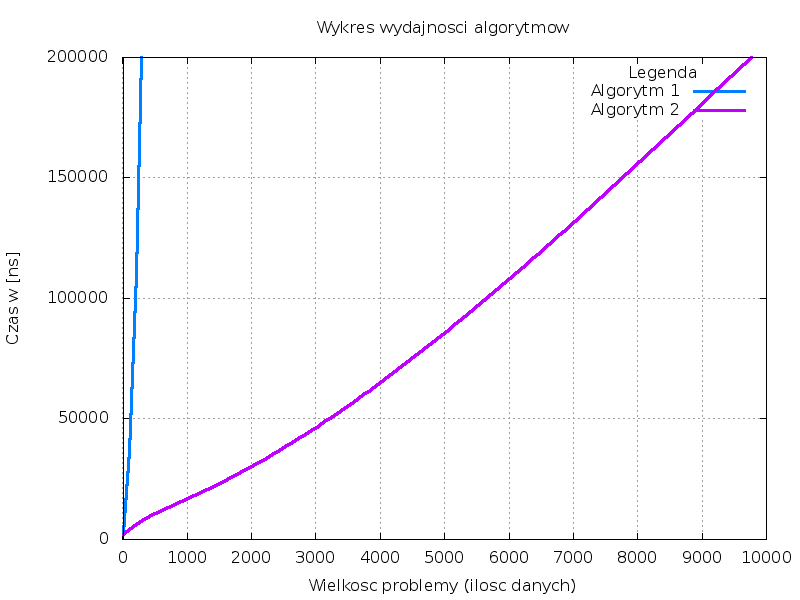
\includegraphics[scale=0.4]{Eksperyment.png}
	\end{center}
\end{figure}
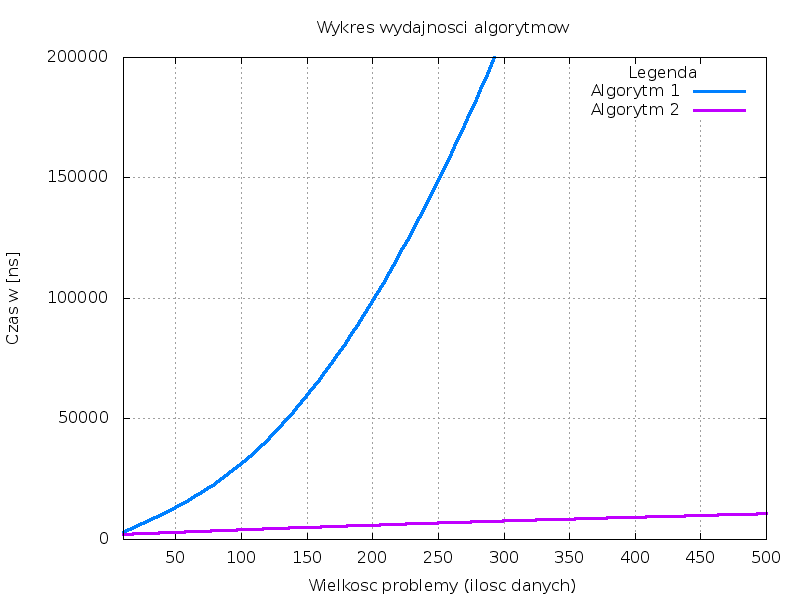
\includegraphics[scale=0.4]{Eksperyment-1.png}
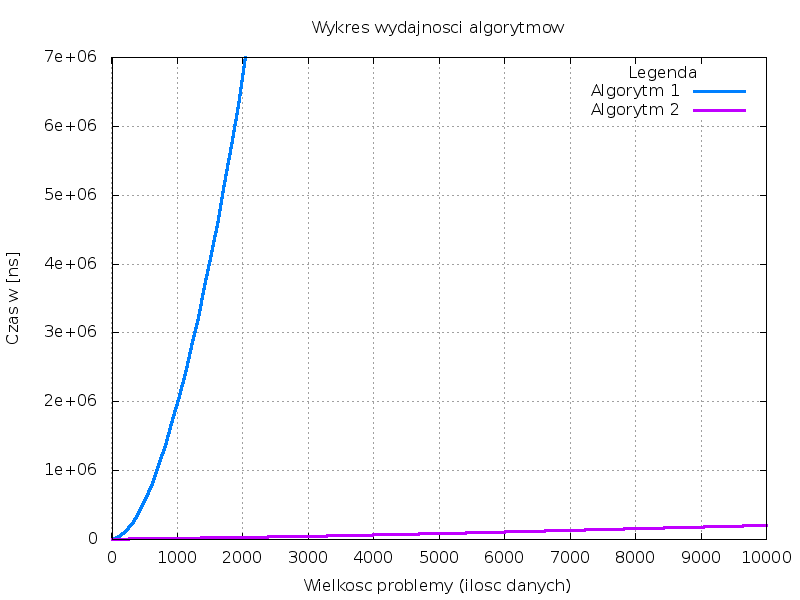
\includegraphics[scale=0.4]{Eksperyment-2.png}
\end{center}

\section{Wnioski}

Wnioski z przeprowadzonej analizy są bardzo proste - algorytm podwajający wielkość
tablicy przy jej przepełnieniu i zwalniający gdy jedna-czwarta jest zajęta
jest o wiele bardziej wydajniejszym i efektywniejszym stosem. Wykres tego algorytmu 
idący niemalże przy osi z pewnością za tym przemawia. Drugi algorytm również
spełnia swoje zadanie, jednak prędko pnie się ku górze, co przemawia na jego 
niekorzyść - oznacza to o wiele dłuższy czas działania dla takiego samego zestawu
danych jak dla algorytmu drugiego, co jest wyraźnie odczuwalne podczas testowania
algorytmów.\\


Próbując odpowiedzieć na pytanie: "Dlaczego akurat drugi algorytm jest lepszy?"
myślę, że zajmowanie nowego kawałka pamięci dla każdego nowego elementu i
zwalnianie jej musi być bardzo obliczenio-chłonne, a przez to o wiele wolniejsze.
Za to rzadkie, acz konkretne zwiększanie pamięci i zwalnianie jej jest wyjściem
optymalnym, pozwalającym na ulepszenie działania mojego stosu.\\\\


\end{document}
